\documentclass[10pt,a4paper]{article}

\usepackage[spanish,es-noshorthands]{babel}
\usepackage[utf8]{inputenc}
\usepackage[T1]{fontenc}
\usepackage{graphicx}
\usepackage[margin=1.6cm]{geometry}
\usepackage{parskip}
\usepackage{booktabs}
\usepackage[font=small]{caption}
\usepackage{hyperref}
\usepackage{amsmath}
\usepackage[table]{xcolor}
\usepackage{fancyhdr}
\usepackage{tikz}
\usetikzlibrary{positioning,shadows,calc,arrows.meta,decorations.pathreplacing}
\usepackage{tcolorbox}
\usepackage{enumitem}

\definecolor{primary}{HTML}{1A5276}
\definecolor{accent}{HTML}{2E86C1}
\definecolor{lightbg}{HTML}{EBF5FB}
\definecolor{darktext}{HTML}{2C3E50}
\definecolor{grayrule}{HTML}{BDC3C7}
\definecolor{success}{HTML}{27AE60}
\definecolor{warning}{HTML}{E67E22}
\definecolor{convblue}{HTML}{3498DB}
\definecolor{poolgreen}{HTML}{2ECC71}
\definecolor{fcorange}{HTML}{E67E22}

\hypersetup{colorlinks=true,linkcolor=accent,urlcolor=accent,citecolor=primary}

\pagestyle{fancy}\fancyhf{}
\fancyhead[L]{\footnotesize\color{accent}\textsc{CNN Anime Faces} \color{grayrule}$\mid$ Aprendizaje Profundo}
\fancyhead[R]{\footnotesize\color{grayrule}\thepage}
\renewcommand{\headrule}{{\color{primary}\hrule height 0.6pt}}
\renewcommand{\footrule}{}

\newtcolorbox{keyfinding}{colback=success!10,colframe=success,boxrule=0.5pt,arc=3pt,fontupper=\small\bfseries}

\begin{document}
\thispagestyle{plain}
\begin{center}
{\Huge\color{primary}\textbf{Clasificación de Rostros Anime}}\\[3pt]
{\Large\color{accent}CNN desde Cero con Clustering No Supervisado}\\[8pt]
{\color{grayrule}\rule{0.4\textwidth}{0.4pt}}
\end{center}
\vspace{-8pt}

% ── ABSTRACT ──
\begin{tcolorbox}[colback=lightbg,colframe=primary,arc=3pt,fontupper=\small]
\textbf{\color{primary}Resumen.} Clasificación de 63{,}565 rostros anime (62$\times$62 px) en 4 categorías semánticas sin etiquetas previas. Pipeline: ResNet18 + K-means para clustering, Gemma~4 para etiquetado semántico, SVM para extrapolación, y CNN VGG-style entrenada desde cero. \textbf{Accuracy: 73.5\%} (2.94$\times$ baseline aleatorio). Se incluye visualización UMAP con regiones, mapas Grad-CAM y análisis de errores.
\end{tcolorbox}

% ── 1. INTRODUCCIÓN ──
\section{Introducción}

El dataset \texttt{anime\_faces} contiene 63{,}565 imágenes JPEG de $62{\times}62$ px sin etiquetas de clase. La clasificación de estos rostros es desafiante por su homogeneidad visual y baja resolución. Trabajos previos en clasificación de rostros utilizan CNN pre-entrenadas con transfer learning~\cite{he2016deep,simonyan2015very}; este trabajo entrena desde cero sobre etiquetas generadas mediante clustering no supervisado.

% ── 2. METODOLOGÍA ──
\section{Metodología}

\subsection{Pipeline y Clustering}
\vspace{-4pt}
\begin{figure}[ht]
\centering
\resizebox{\textwidth}{!}{%
\begin{tikzpicture}[
  node distance=1.1cm,
  block/.style={rectangle, draw=primary, fill=lightbg, text=darktext,
    rounded corners=3pt, minimum width=2.4cm, minimum height=0.75cm,
    font=\small\bfseries, align=center, drop shadow={opacity=0.12}},
  arrow/.style={->, >=Stealth, line width=1.2pt, color=accent},
]
\node[block,fill=primary!15] (data) {Dataset\\{\normalfont\tiny 63k imgs}};
\node[block,right=of data] (resnet) {ResNet18\\{\normalfont\tiny 512-d feats}};
\node[block,right=of resnet] (kmeans) {K-Means\\{\normalfont\tiny $k{=}4$}};
\node[block,right=of kmeans] (gemma) {Gemma 4\\{\normalfont\tiny Etiquetas}};
\node[block,below=1.2cm of kmeans] (svm) {SVM\\{\normalfont\tiny Extrapol.}};
\node[block,right=of gemma] (cnn) {CNN\\{\normalfont\tiny Entrena}};
\node[block,right=of cnn,fill=accent!20] (out) {Clasificador\\{\normalfont\tiny\bfseries 73.5\%}};
\draw[arrow] (data) -- (resnet);
\draw[arrow] (resnet) -- (kmeans);
\draw[arrow] (kmeans) -- (gemma);
\draw[arrow] (kmeans) -- (svm);
\draw[arrow] (svm) -- (cnn);
\draw[arrow] (cnn) -- (out);
\end{tikzpicture}%
}
\caption{Pipeline: clustering $\to$ etiquetado $\to$ extrapolación $\to$ clasificación.}
\label{fig:pipeline}
\end{figure}
\vspace{-4pt}

Se extrajeron embeddings ResNet18 (512-d) de 200 imágenes aleatorias. K-means ($k=4$, silueta 0.067) agrupó las muestras. La imagen compuesta se envió a Gemma~4~\cite{gemma42024} para etiquetado semántico (Tabla~\ref{tab:labels}). Un SVM (RBF, $C=10$) extrapoló las etiquetas a 63k imágenes con 100\% de acierto en entrenamiento.

\begin{table}[ht]
\centering\small
\caption{Etiquetas semánticas asignadas por Gemma~4.}
\begin{tabular}{cl}
\toprule
\textbf{Cluster} & \textbf{Etiqueta y descripción} \\
\midrule
1 & \textbf{Soft Bright} --- Rasgos suaves, colores pastel, estética tierna \\
2 & \textbf{Standard Diverse} --- Anime clásico, variedad de diseños y expresiones \\
3 & \textbf{Mature Intense} --- Rasgos definidos, tonos profundos, apariencia dramática \\
4 & \textbf{Edgy Cool} --- Tonos oscuros, diseños modernos con actitud \\
\bottomrule
\end{tabular}
\label{tab:labels}
\end{table}

\begin{figure}[ht]
\centering
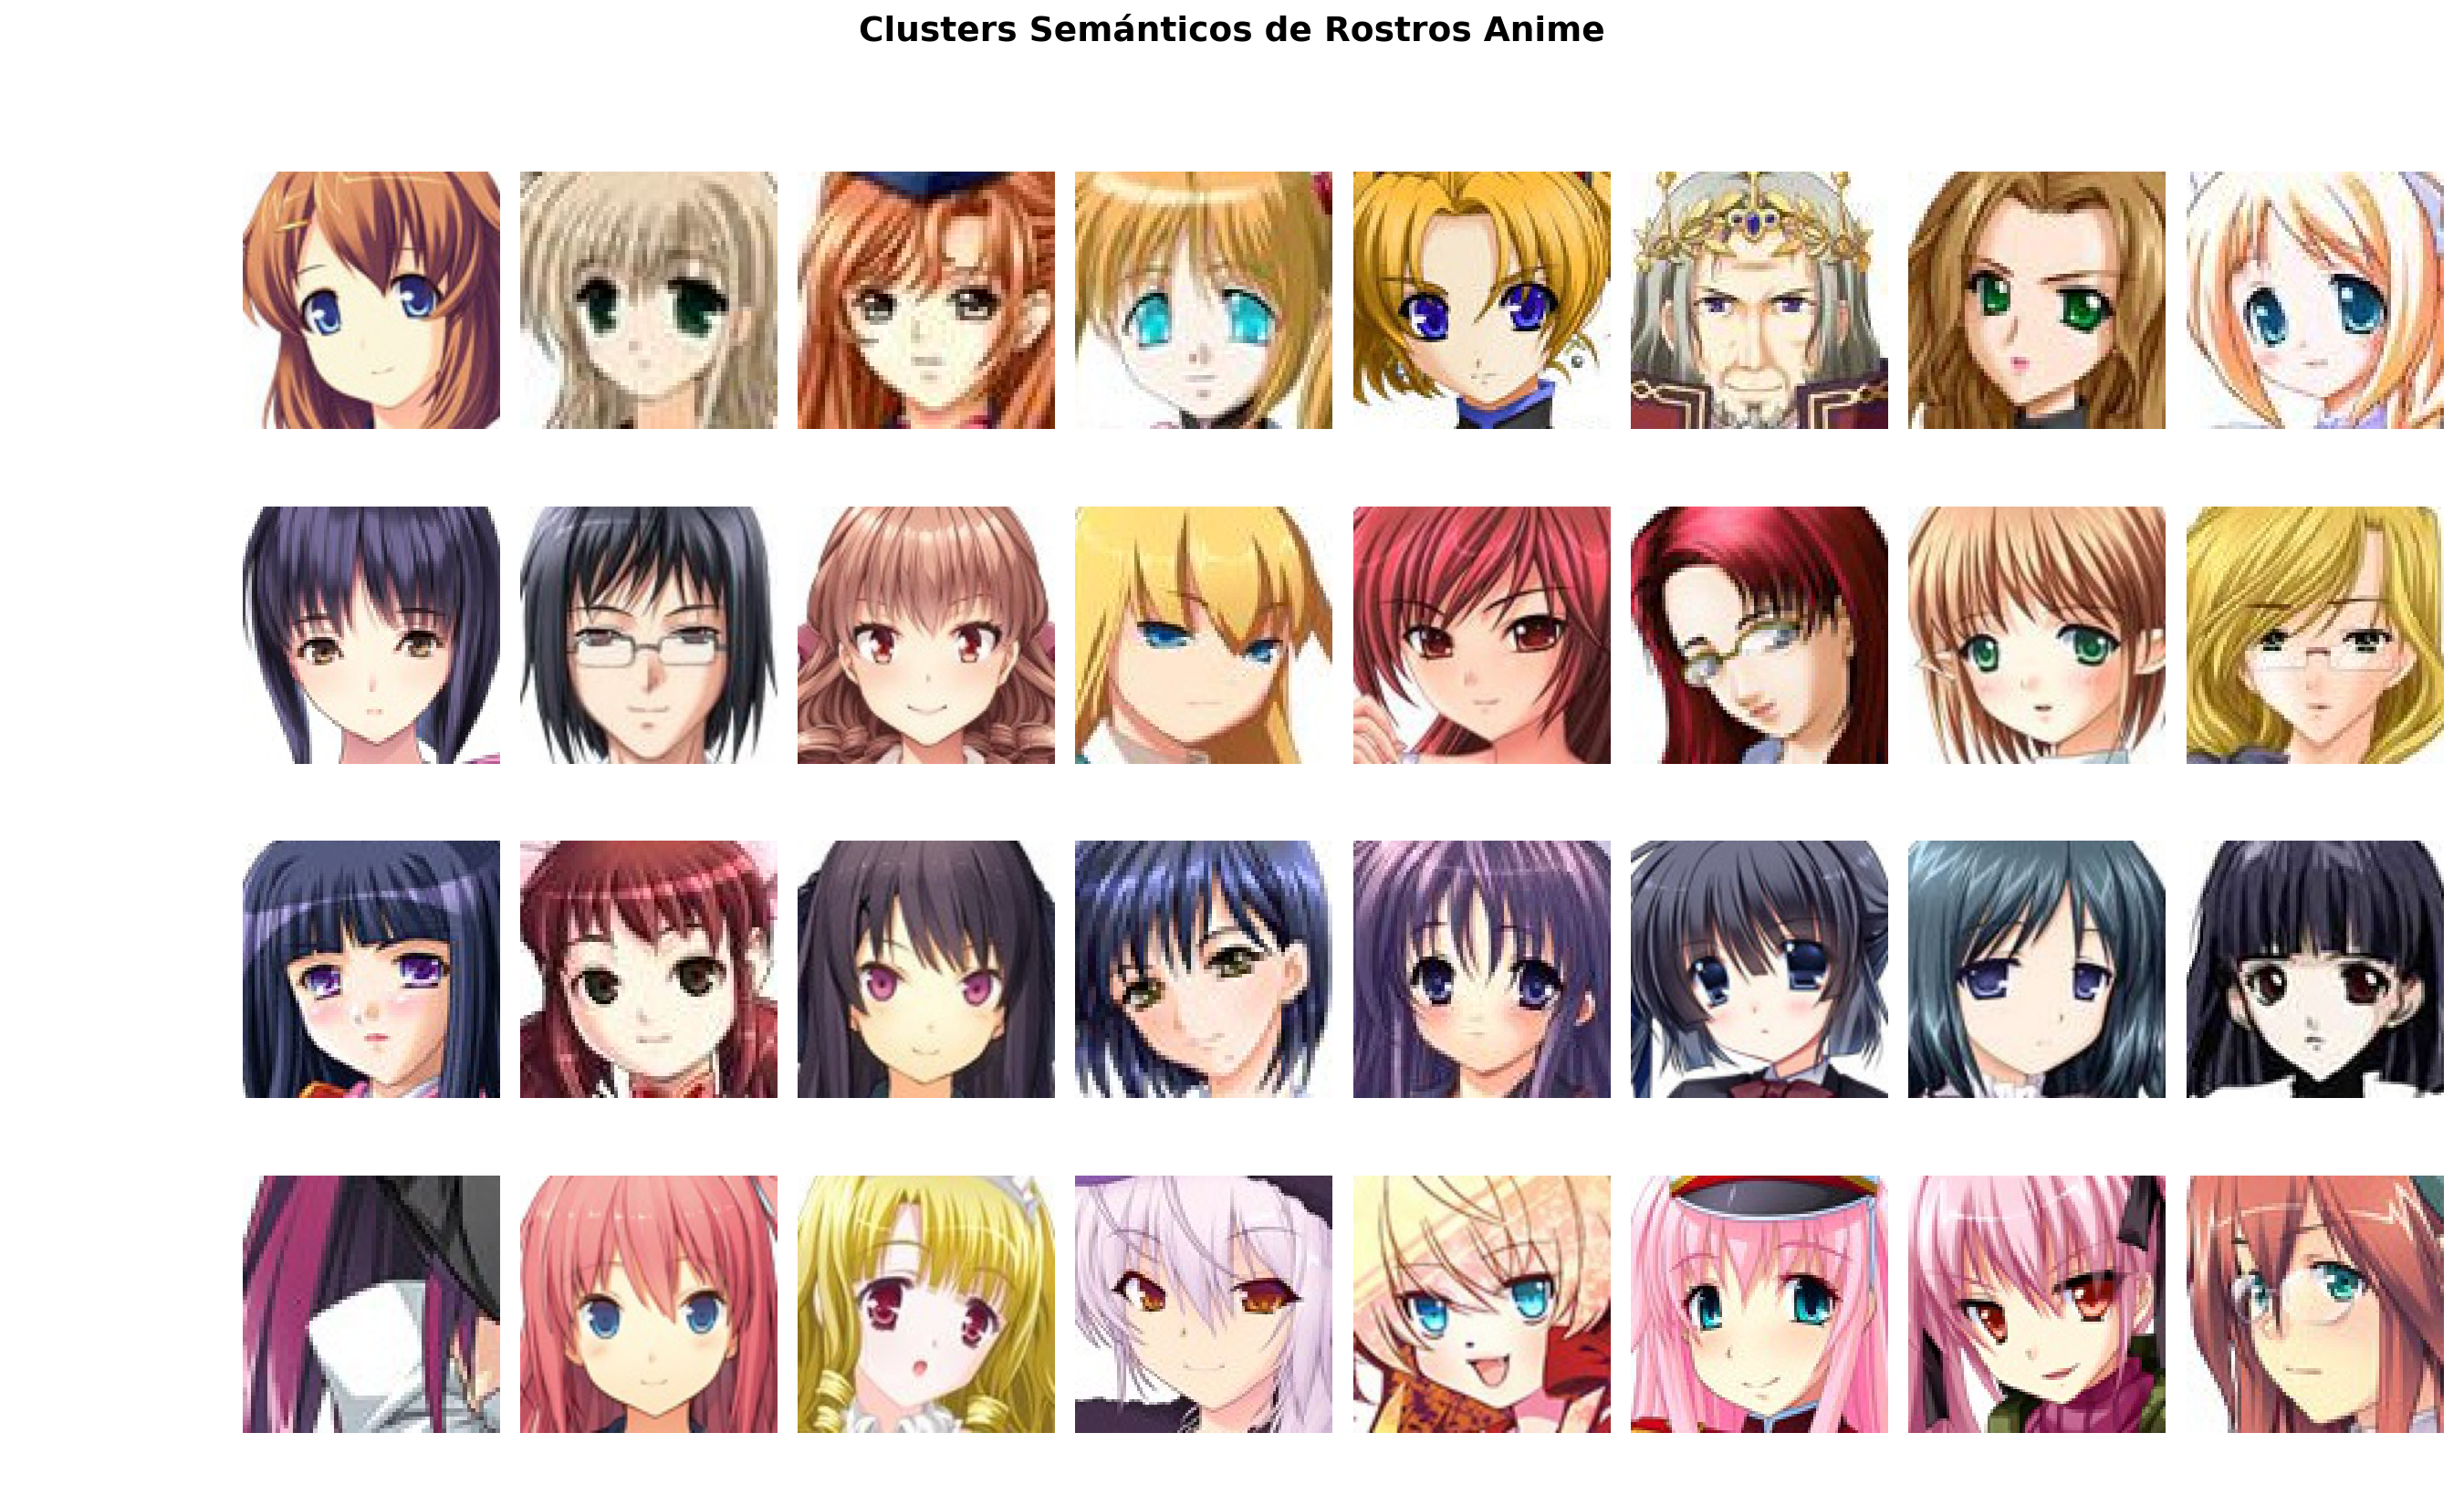
\includegraphics[width=0.65\textwidth]{figuras/clusters_annotated.png}
\caption{Muestras de cada cluster. Etiquetas Gemma~4 y tamaño en la muestra de 200.}
\label{fig:clusters}
\end{figure}

\subsection{Arquitectura CNN}

CNN VGG-style con 4 bloques convolucionales (doble Conv2D $3{\times}3$ + BatchNorm + ReLU + MaxPool $2{\times}2$), aplanamiento a 4096-d, y clasificador FC (Dropout 0.4, 4096$\to$256$\to$4). Total: 2.22M parámetros.

\begin{figure}[ht]
\centering\footnotesize
\resizebox{\textwidth}{!}{%
\begin{tikzpicture}[
  tensor/.style={rectangle, draw=primary!60, fill=primary!5, minimum width=2.5cm,
    minimum height=0.55cm, text=darktext, font=\tiny\ttfamily, align=center, rounded corners=2pt},
  pool/.style={rectangle, draw=poolgreen!70, fill=poolgreen!8,
    minimum width=2.5cm, minimum height=0.45cm, font=\tiny, align=center, rounded corners=2pt},
  fc/.style={rectangle, draw=fcorange!70, fill=fcorange!8,
    minimum width=1.6cm, minimum height=0.7cm, font=\tiny, align=center, rounded corners=2pt},
  arr/.style={->, >=Stealth, line width=0.8pt, color=accent},
  brace/.style={decorate,decoration={brace,amplitude=5pt},line width=0.8pt,color=convblue}
]
\node[tensor,fill=primary!10] (inp) {Input: $3{\times}64{\times}64$};
\node[tensor,below=0.25cm of inp] (b1a) {Conv $3{\to}32$ BN ReLU};
\node[tensor,below=0.12cm of b1a] (b1b) {Conv $32{\to}32$ BN ReLU};
\node[pool,below=0.12cm of b1b] (b1p) {MaxPool $\to 32{\times}32{\times}32$};
\node[tensor,below=0.3cm of b1p] (b2a) {Conv $32{\to}64$ BN ReLU};
\node[tensor,below=0.12cm of b2a] (b2b) {Conv $64{\to}64$ BN ReLU};
\node[pool,below=0.12cm of b2b] (b2p) {MaxPool $\to 64{\times}16{\times}16$};
\node[tensor,below=0.3cm of b2p] (b3a) {Conv $64{\to}128$ BN ReLU};
\node[tensor,below=0.12cm of b3a] (b3b) {Conv $128{\to}128$ BN ReLU};
\node[pool,below=0.12cm of b3b] (b3p) {MaxPool $\to 128{\times}8{\times}8$};
\node[tensor,below=0.3cm of b3p] (b4a) {Conv $128{\to}256$ BN ReLU};
\node[tensor,below=0.12cm of b4a] (b4b) {Conv $256{\to}256$ BN ReLU};
\node[pool,below=0.12cm of b4b] (b4p) {MaxPool $\to 256{\times}4{\times}4$};
\node[tensor,fill=primary!8,below=0.3cm of b4p] (flat) {Flatten: $256{\times}4{\times}4 = 4096$};
\node[fc,below=0.25cm of flat] (fc1) {Drop 0.4\\FC 4096$\to$256\\ReLU};
\node[fc,right=0.5cm of fc1] (fc2) {Drop 0.4\\FC 256$\to$4};
\node[tensor,fill=accent!12,right=0.5cm of fc2,minimum width=1.8cm] (out) {Softmax\\{\small 4 clases}};
\draw[arr] (inp) -- (b1a);
\draw[arr] (b1p) -- (b2a); \draw[arr] (b2p) -- (b3a); \draw[arr] (b3p) -- (b4a);
\draw[arr] (b4p) -- (flat); \draw[arr] (flat) -- (fc1);
\draw[arr] (fc1) -- (fc2); \draw[arr] (fc2) -- (out);
\draw[brace] ([xshift=-0.8cm]b1a.north west) -- ([xshift=-0.8cm]b1p.south west)
  node[midway,left=0.35cm,font=\tiny\color{convblue}]{B1};
\draw[brace] ([xshift=-0.8cm]b2a.north west) -- ([xshift=-0.8cm]b2p.south west)
  node[midway,left=0.35cm,font=\tiny\color{convblue}]{B2};
\draw[brace] ([xshift=-0.8cm]b3a.north west) -- ([xshift=-0.8cm]b3p.south west)
  node[midway,left=0.35cm,font=\tiny\color{convblue}]{B3};
\draw[brace] ([xshift=-0.8cm]b4a.north west) -- ([xshift=-0.8cm]b4p.south west)
  node[midway,left=0.35cm,font=\tiny\color{convblue}]{B4};
\end{tikzpicture}%
}
\caption{Arquitectura CNN (2.22M parámetros). \textcolor{convblue}{$\bullet$} B1--B4 = bloques convolucionales. \textcolor{poolgreen}{$\bullet$} MaxPool. \textcolor{fcorange}{$\bullet$} FC.}
\label{fig:cnn}
\end{figure}

\noindent\textbf{Entrenamiento:} Adam ($\text{lr}=10^{-3}$), batch 128, 20 épocas, early stopping (paciencia 7), ReduceLROnPlateau. Data augmentation: HorizontalFlip, ColorJitter(0.1), Rotation($\pm5^\circ$). Normalización $[-1,1]$. Split 70/15/15\%. GPU: RTX 3070 8GB. PyTorch~\cite{pytorch} + scikit-learn~\cite{pedregosa2011scikit}.

% ── 3. RESULTADOS ──
\section{Resultados}

\begin{figure}[ht]
\centering
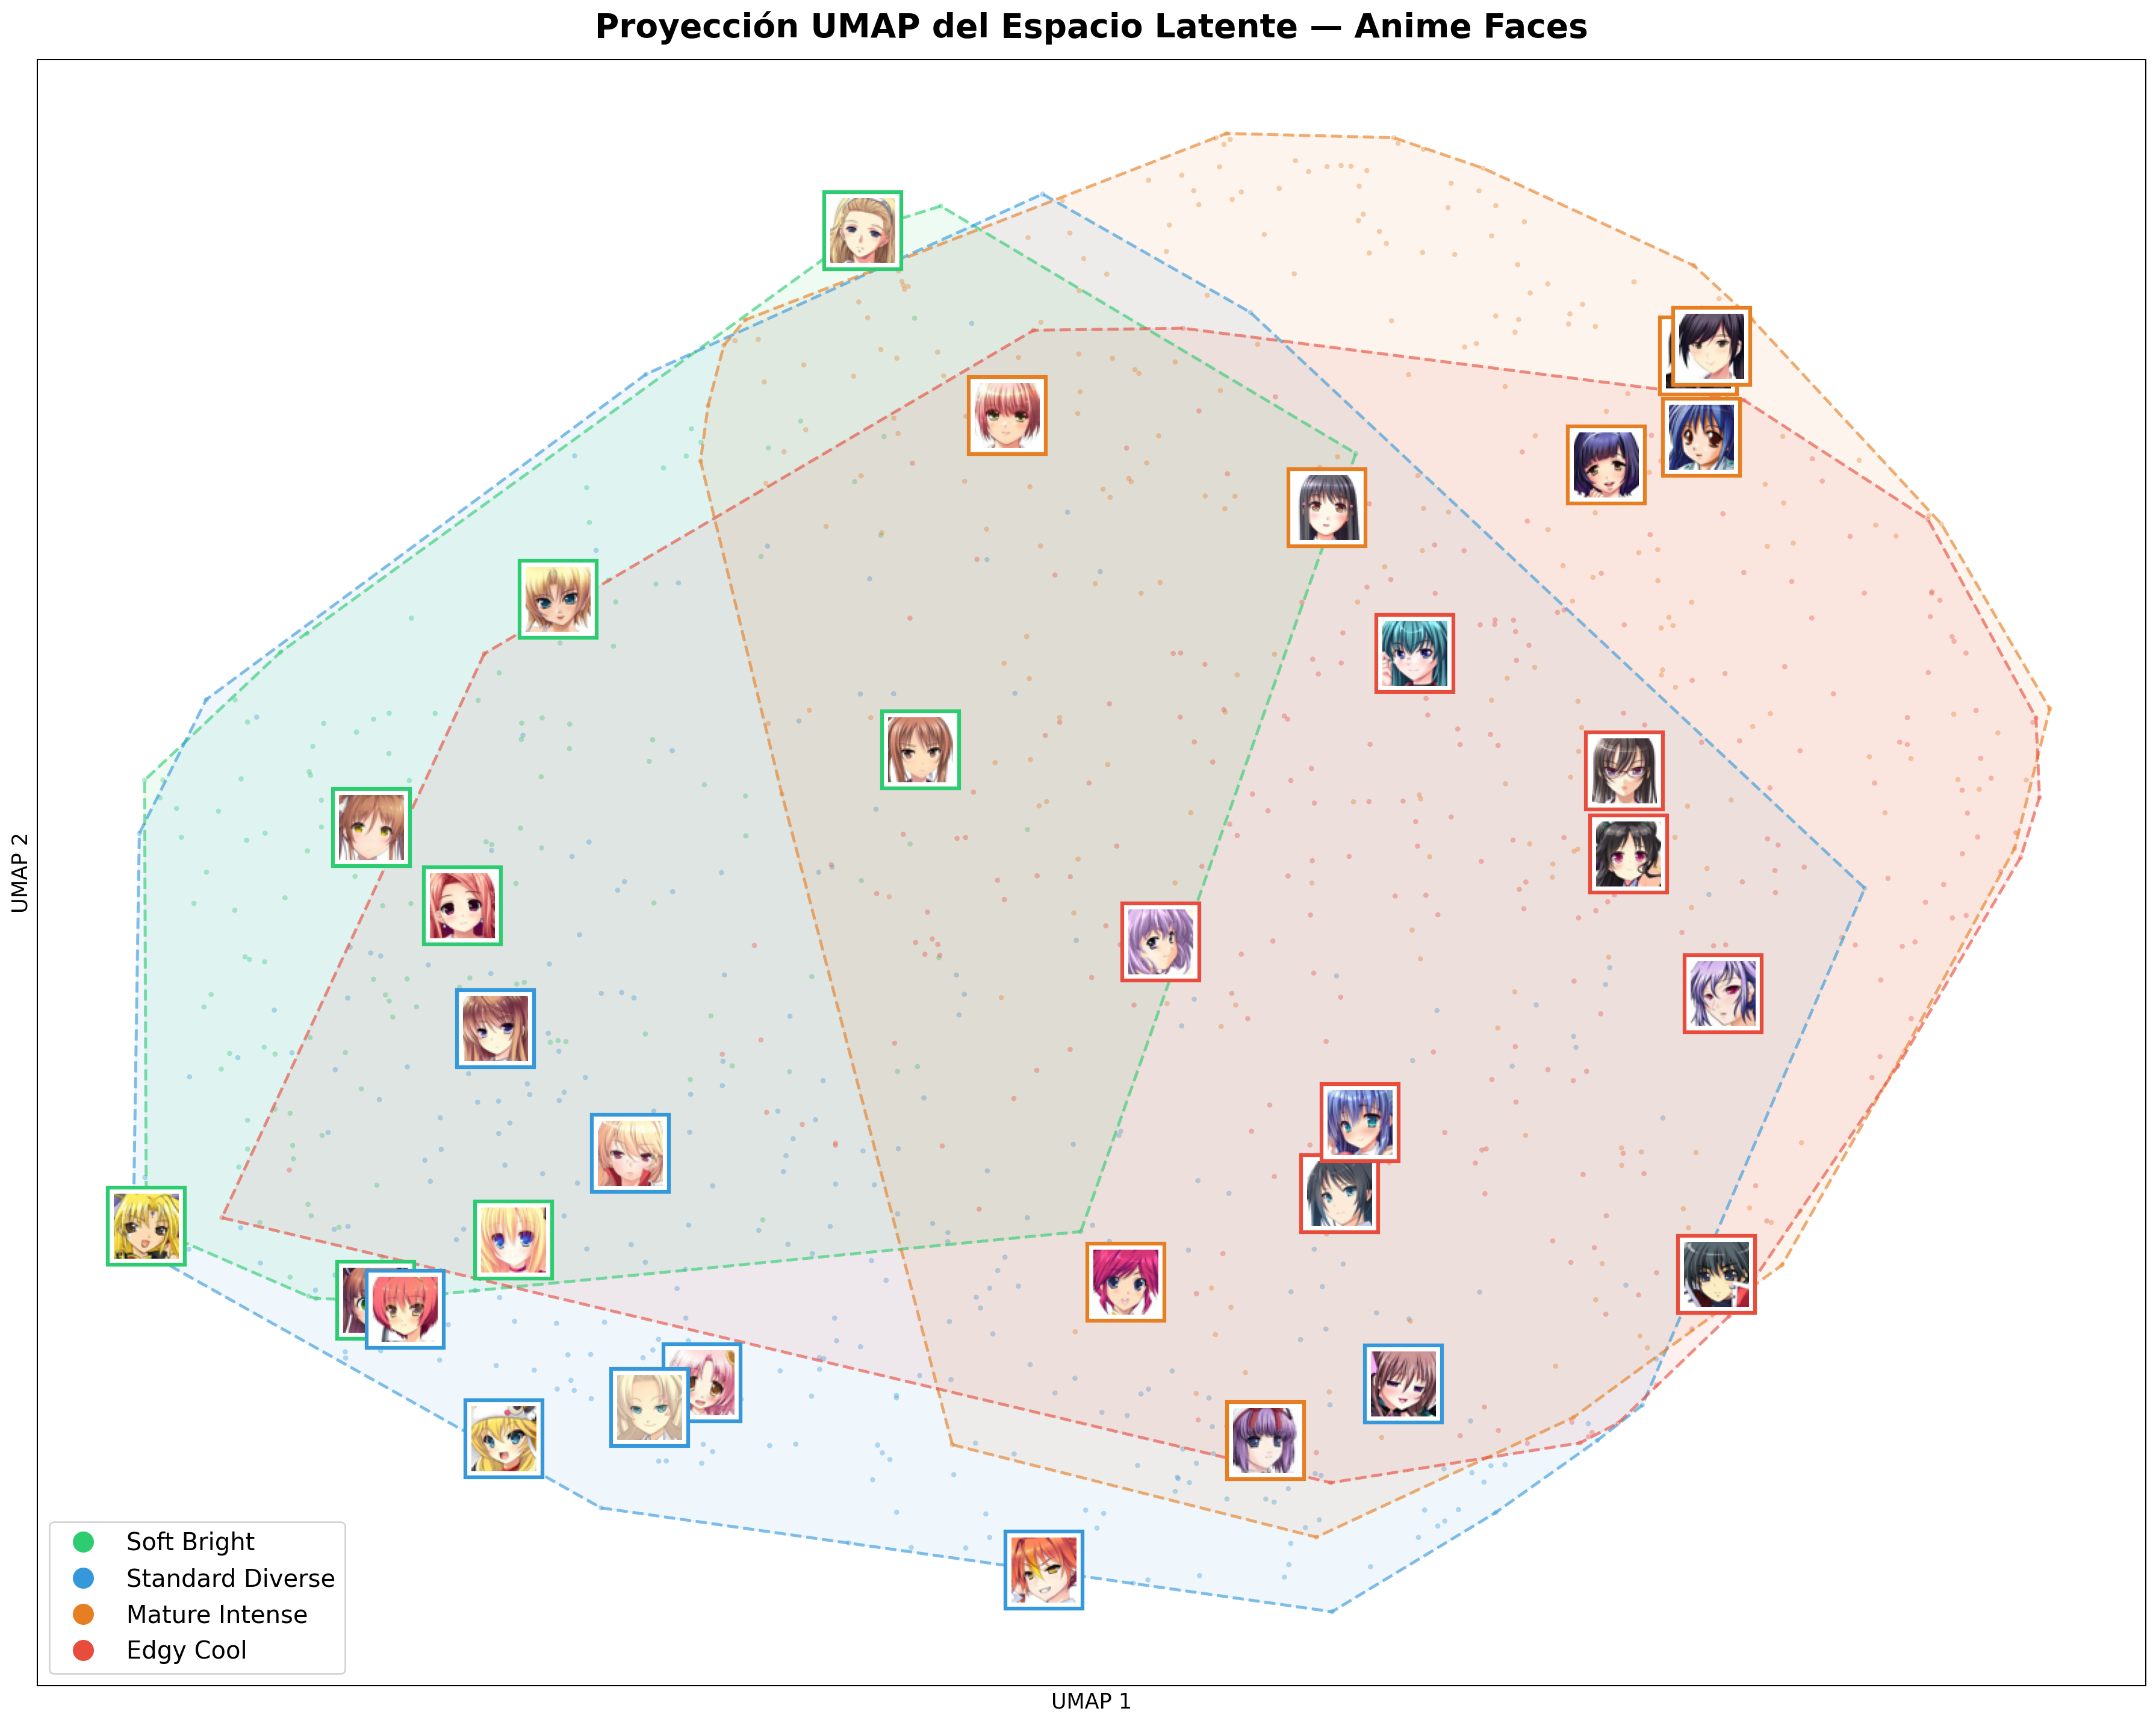
\includegraphics[width=0.75\textwidth]{figuras/umap_projection.png}
\caption{Proyección UMAP de 1{,}000 rostros con regiones Convex Hull por categoría. Miniaturas $4{\times}8$ en coordenadas proyectadas. Soft Bright (verde) y Edgy Cool (rojo) ocupan regiones opuestas; Standard Diverse (azul) y Mature Intense (naranja) se solapan parcialmente.}
\label{fig:umap}
\end{figure}

\begin{figure}[ht]
\centering
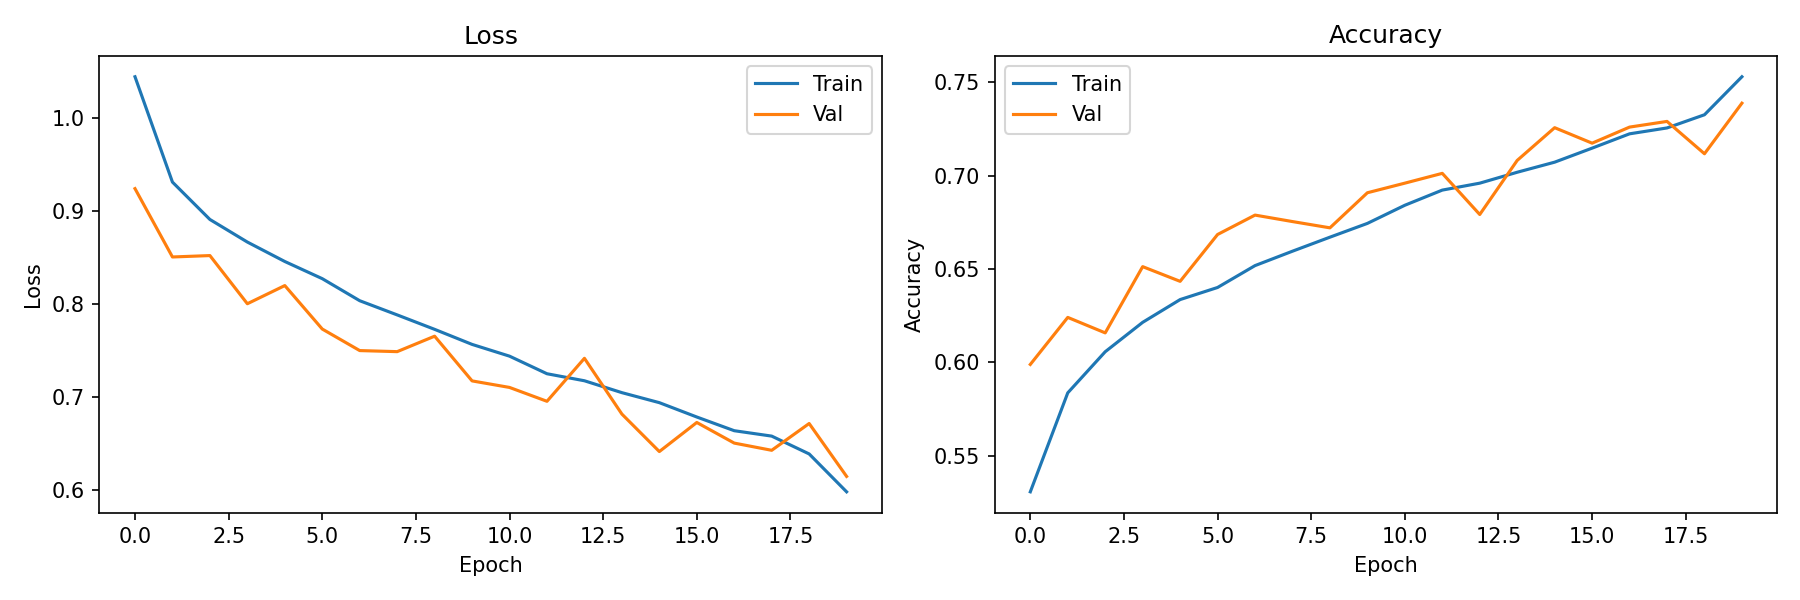
\includegraphics[width=0.58\textwidth]{figuras/training_curves.png}
\caption{Curvas de entrenamiento. Val loss mínimo: 0.614 en época 20.}
\label{fig:curves}
\end{figure}

\begin{table}[ht]
\centering\small
\caption{Métricas por clase en test (9{,}536 imágenes). Baseline aleatorio: 25\%.}
\begin{tabular}{lrrr}
\toprule
\textbf{Categoría} & \textbf{Precision} & \textbf{Recall} & \textbf{F1} \\
\midrule
Soft Bright       & 0.617 & \textbf{0.816} & 0.702 \\
Standard Diverse  & 0.799 & 0.720 & 0.758 \\
Mature Intense    & \textbf{0.814} & 0.654 & 0.725 \\
Edgy Cool         & 0.686 & 0.807 & 0.741 \\
\midrule
\textbf{Accuracy} & \multicolumn{3}{c}{\textbf{73.50\%} (2.94$\times$ baseline)} \\
\bottomrule
\end{tabular}
\label{tab:metrics}
\end{table}

\begin{keyfinding}
La CNN supera en $\mathbf{2.94\times}$ al clasificador aleatorio (73.5\% vs.\ 25\%), validando que los clusters no supervisados contienen información discriminativa suficiente.
\end{keyfinding}

\begin{figure}[ht]
\centering
\begin{minipage}{0.48\textwidth}
\centering
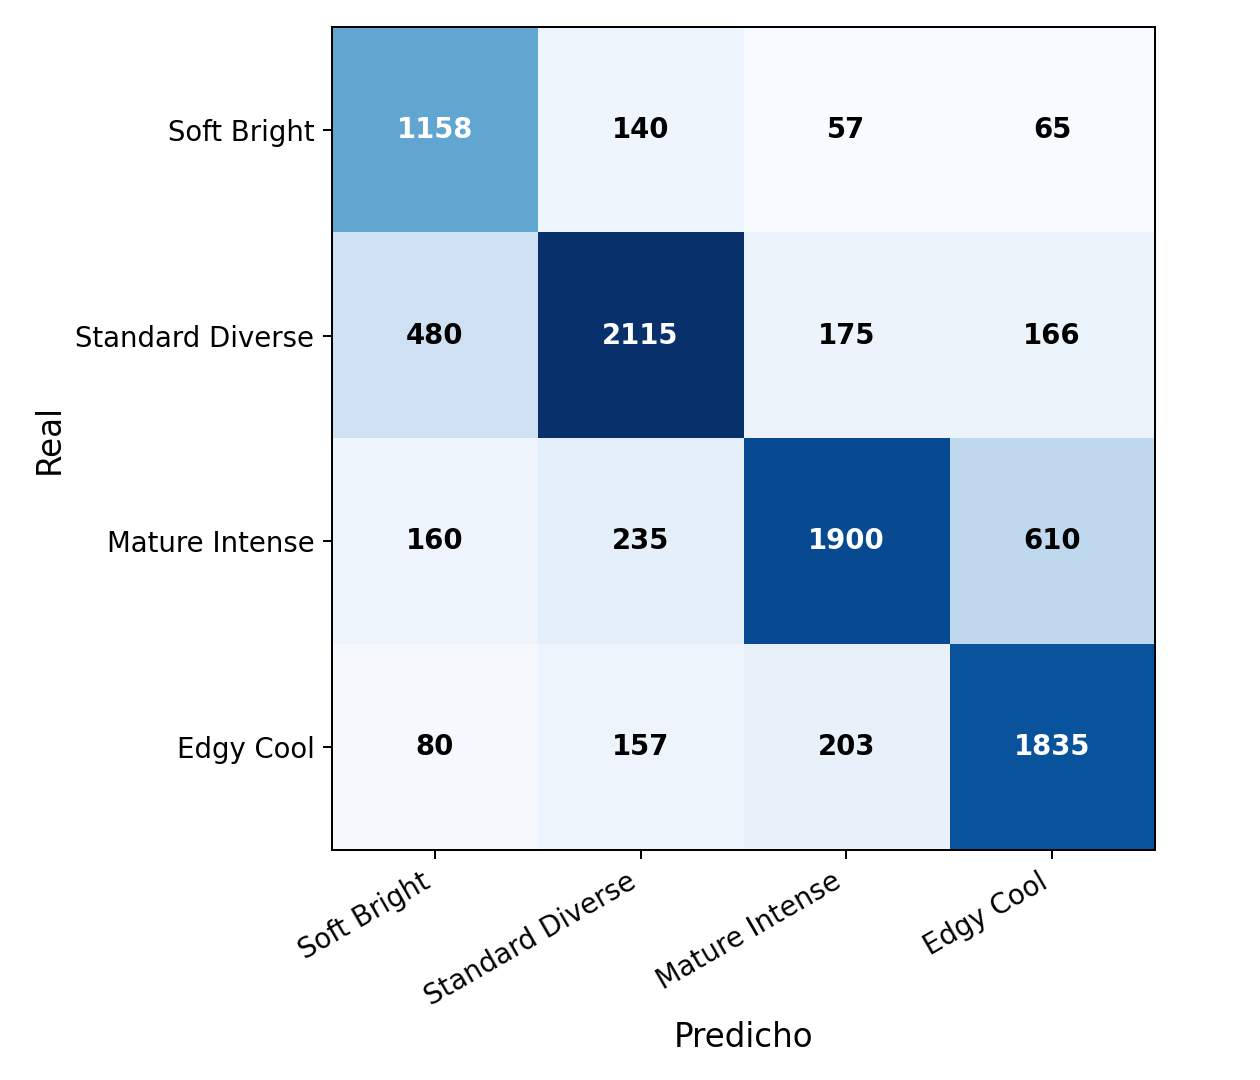
\includegraphics[width=\textwidth]{figuras/confusion_matrix.png}
\captionof{figure}{Matriz de confusión. Las confusiones ocurren entre categorías adyacentes (Standard Diverse $\leftrightarrow$ Mature Intense).}
\label{fig:confusion}
\end{minipage}\hfill
\begin{minipage}{0.48\textwidth}
\centering
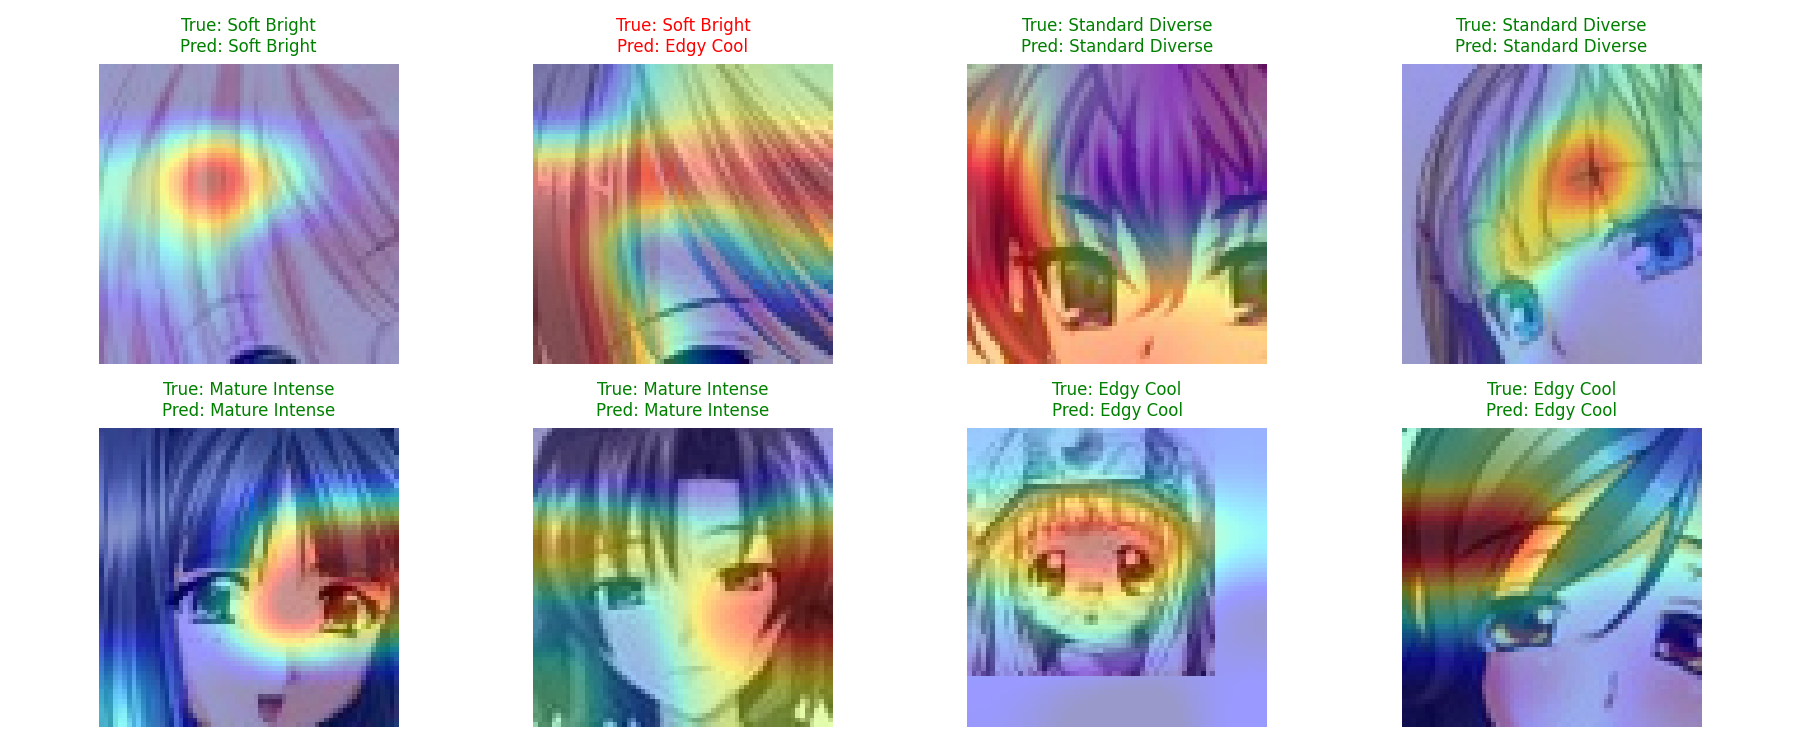
\includegraphics[height=4.4cm]{figuras/gradcam.png}
\captionof{figure}{Mapas Grad-CAM. La CNN atiende la región facial central (ojos, nariz, boca), confirmando aprendizaje de features discriminativos.}
\label{fig:gradcam}
\end{minipage}
\end{figure}

\begin{figure}[ht]
\centering
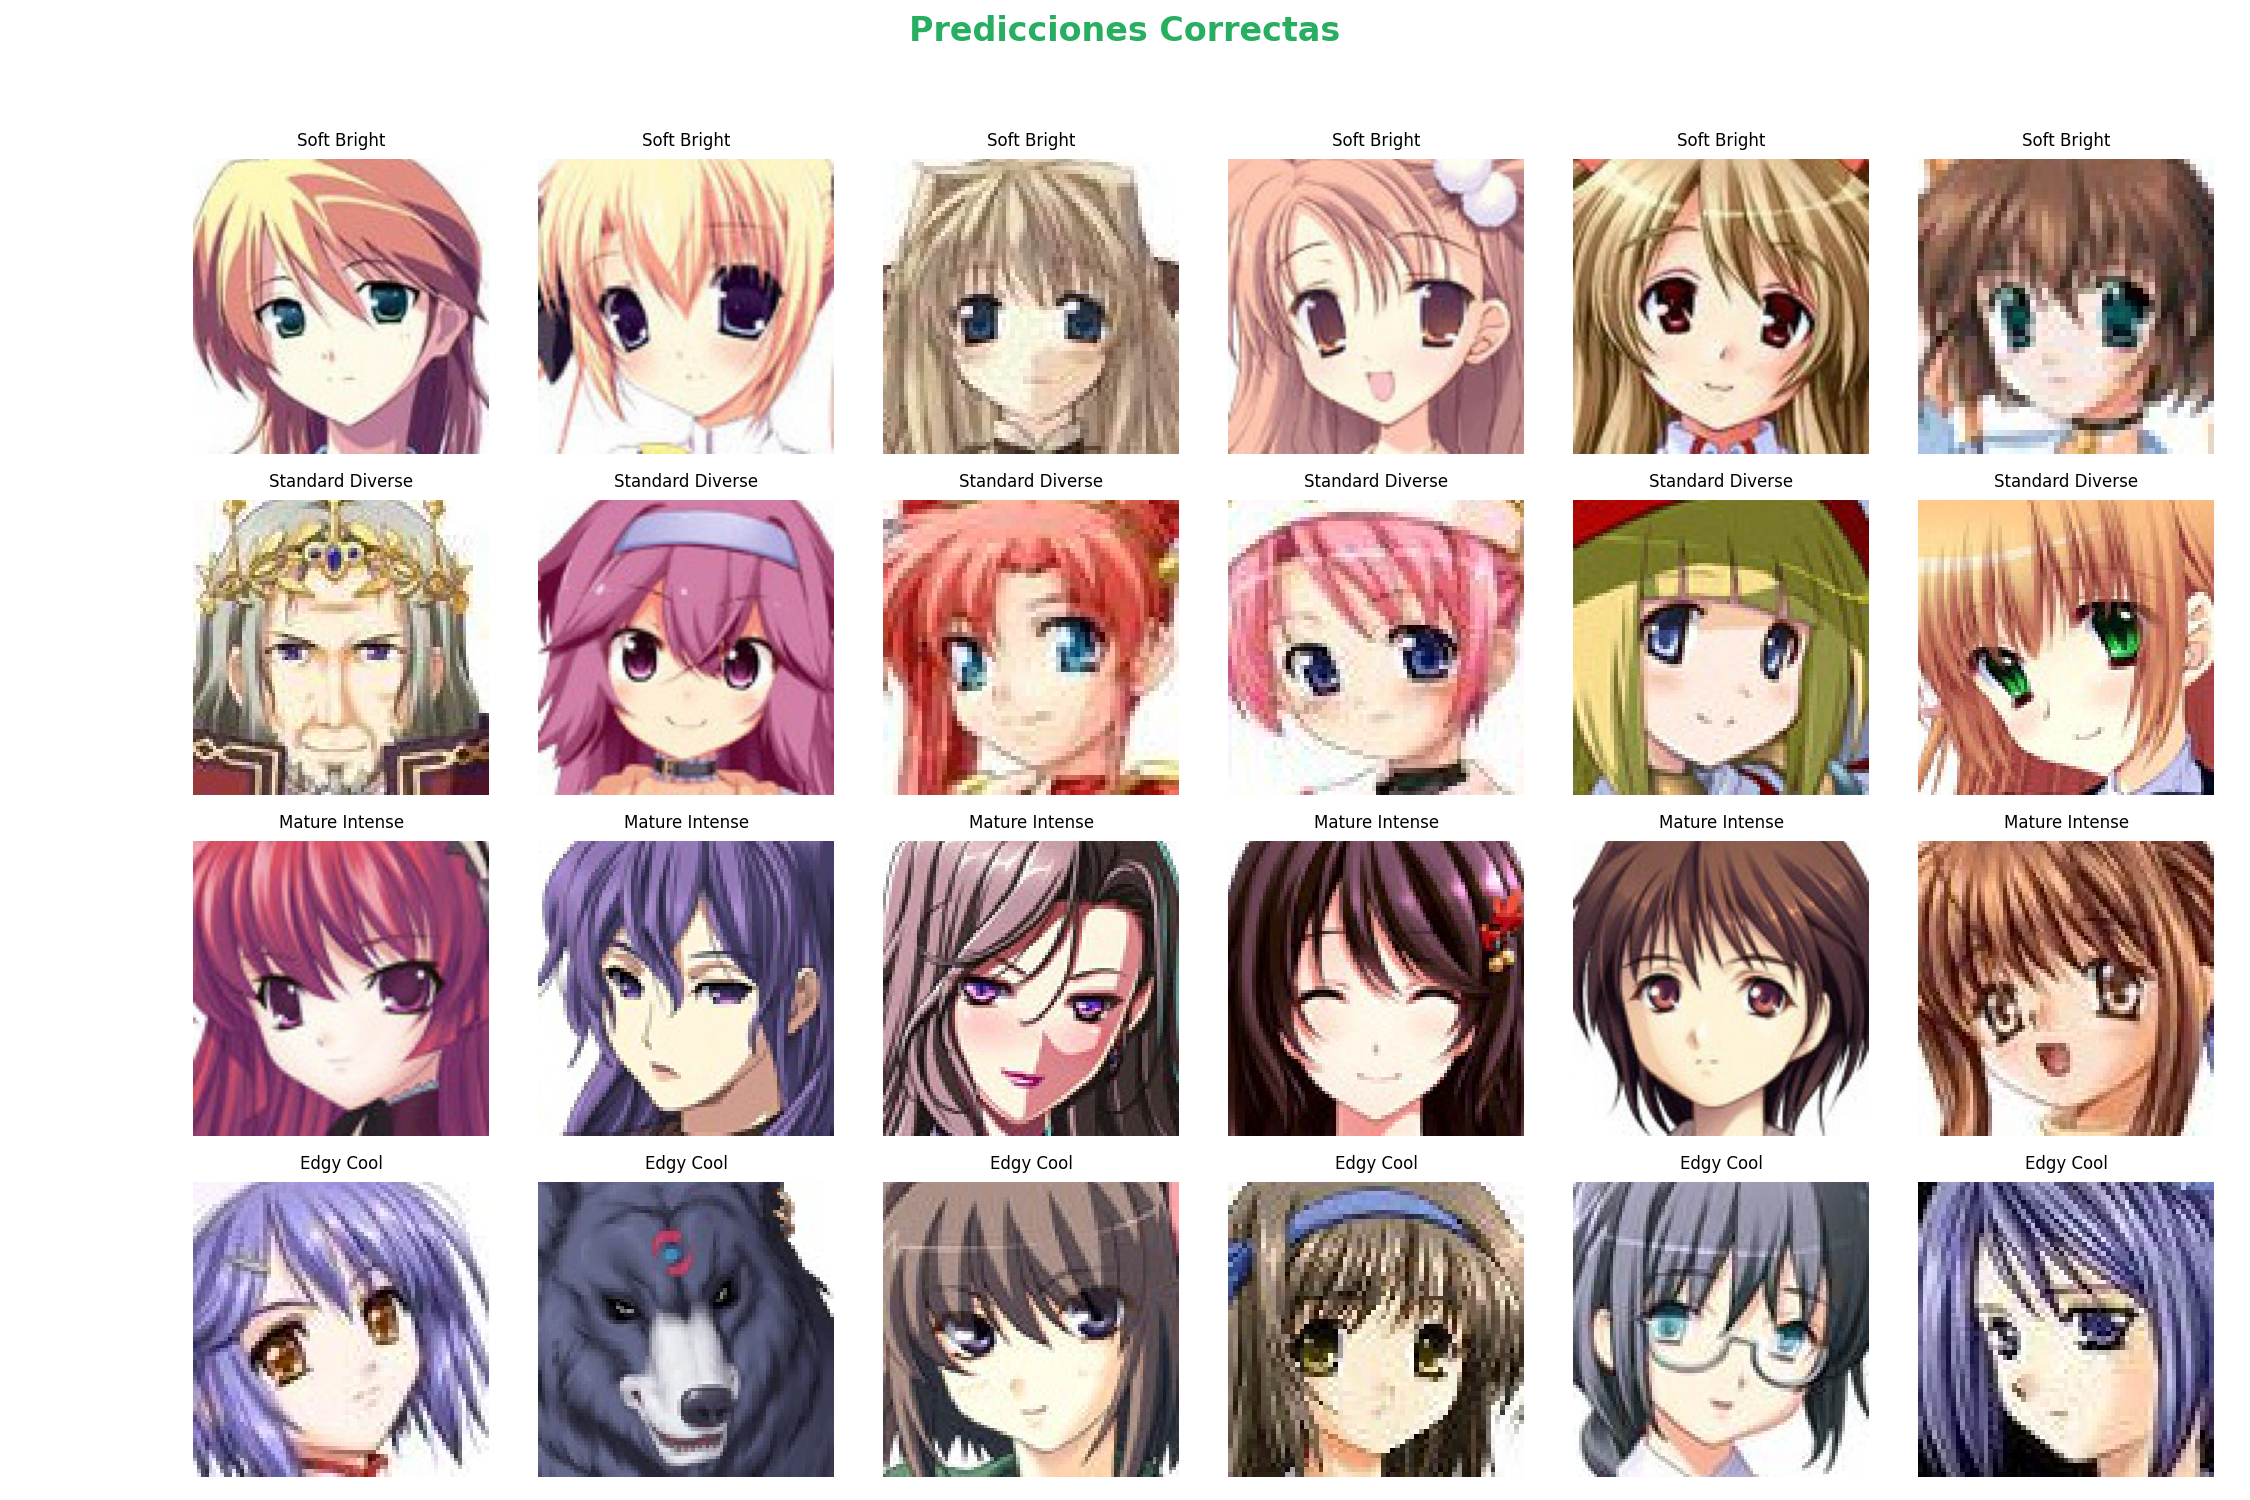
\includegraphics[width=0.92\textwidth]{figuras/inference_correct.png}
\caption{Predicciones correctas (7{,}008/9{,}536). Filas: clases reales.}
\label{fig:correct}
\end{figure}
\vspace{-8pt}
\begin{figure}[ht]
\centering
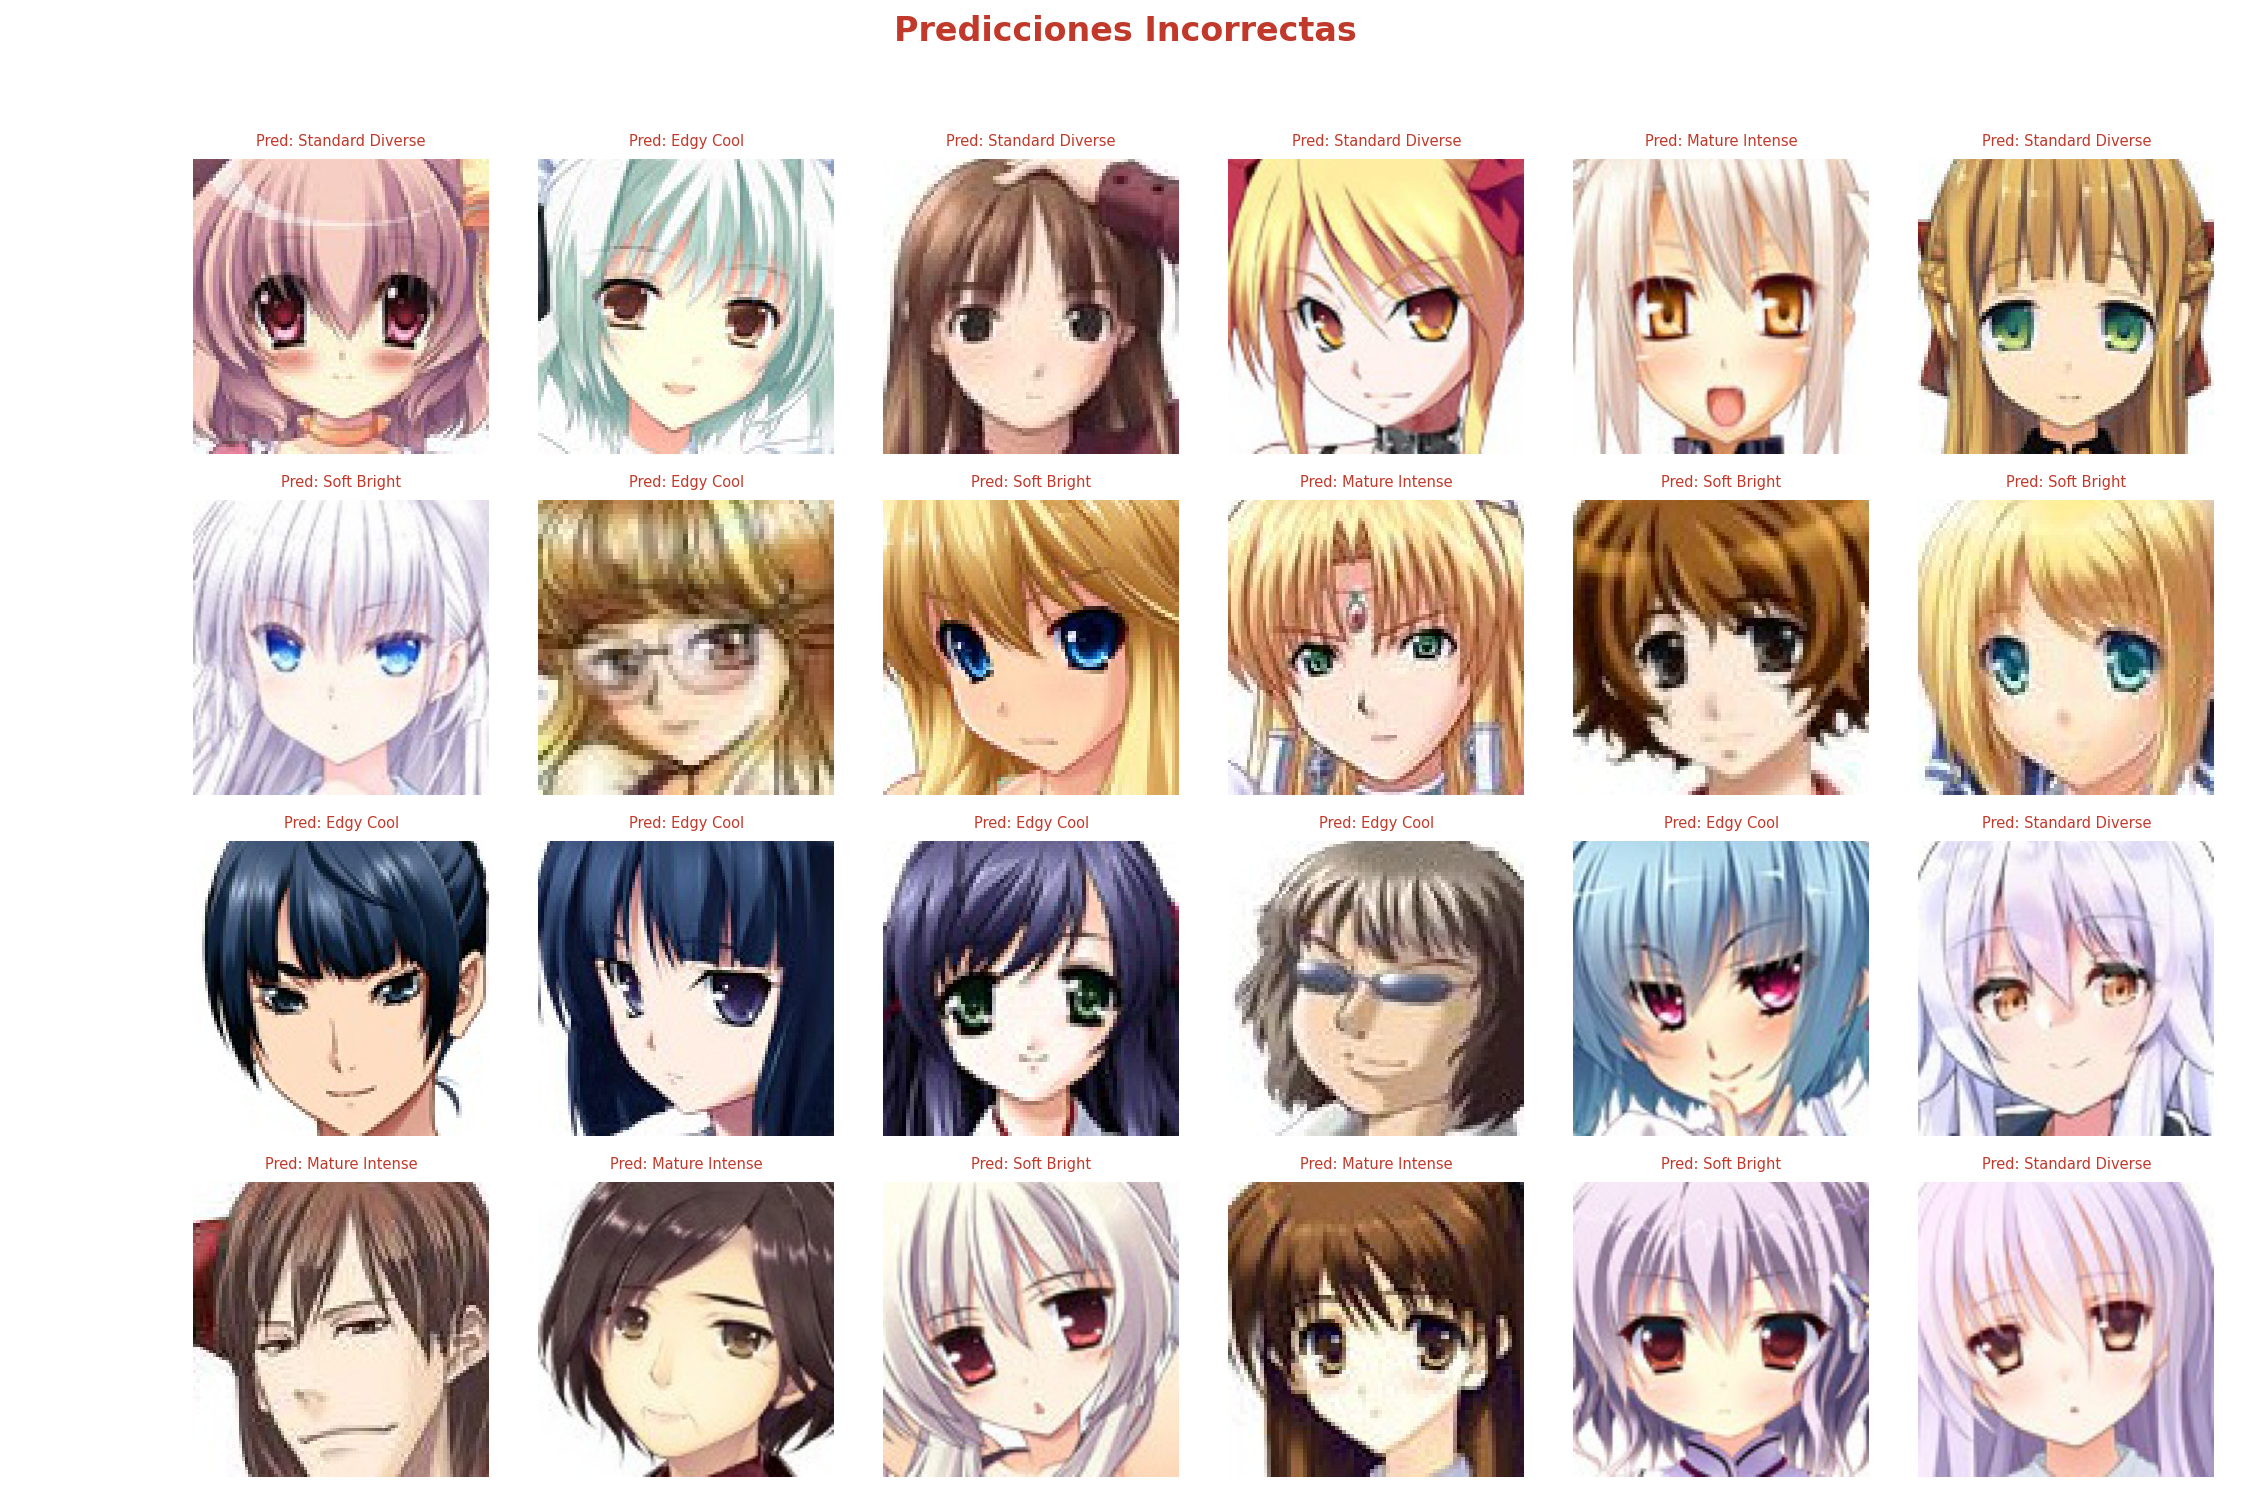
\includegraphics[width=0.92\textwidth]{figuras/inference_incorrect.png}
\caption{Predicciones incorrectas (2{,}528/9{,}536). Errores por iluminación o rasgos ambiguos.}
\label{fig:incorrect}
\end{figure}

% ── 4. CONCLUSIONES ──
\section{Conclusiones}

\begin{enumerate}[leftmargin=*,itemsep=2pt]
\item \textbf{Clustering efectivo:} ResNet18 + K-means genera 4 categorías visualmente coherentes, enriquecidas semánticamente por Gemma~4 (Soft Bright, Standard Diverse, Mature Intense, Edgy Cool).
\item \textbf{Extrapolación eficiente:} SVM etiqueta 63k imágenes en segundos con 100\% de consistencia en entrenamiento.
\item \textbf{CNN competitiva:} Arquitectura VGG-style de 2.22M parámetros alcanza 73.5\% de accuracy (2.94$\times$ baseline) en 20 épocas.
\item \textbf{Interpretabilidad:} Grad-CAM confirma atención en regiones faciales; UMAP revela separación espacial entre categorías opuestas.
\end{enumerate}

\noindent\textbf{Trabajo futuro:} explorar $k>4$, arquitecturas residuales, y data augmentation avanzado (MixUp, CutMix) para mejorar robustez.

\bibliographystyle{plain}
\bibliography{bibliografia}

\end{document}
